\documentclass{standalone}
\usepackage{preset}
\begin{document}
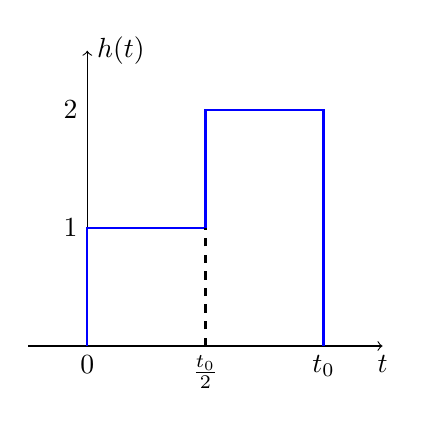
\begin{tikzpicture}[x=15mm,y=15mm]
    \draw[->](-.5,0)--(2.5,0)node[below]{\(t\)};
    \draw[->](0,0)--(0,2.5)node[right]{\(h(t)\)};
    \foreach \x/\label in {0/\(0\),1/\(\frac{t_0}2\),2/\(t_0\)}{
        \draw(\x,0)node[below]{\label};
    }
    \draw(0,1)node[left]{\(1\)};
    \draw(0,2)node[left]{\(2\)};
    \draw[blue,thick](0,0)--(0,1)--(1,1)--(1,2)--(2,2)--(2,0);
    \draw[dashed,thick](1,0)--(1,1);
\end{tikzpicture}
\end{document}
